\subsubsection{Joining a Session}

\begin{figure}[H]
	\begin{subfigure}{0.70\linewidth}
		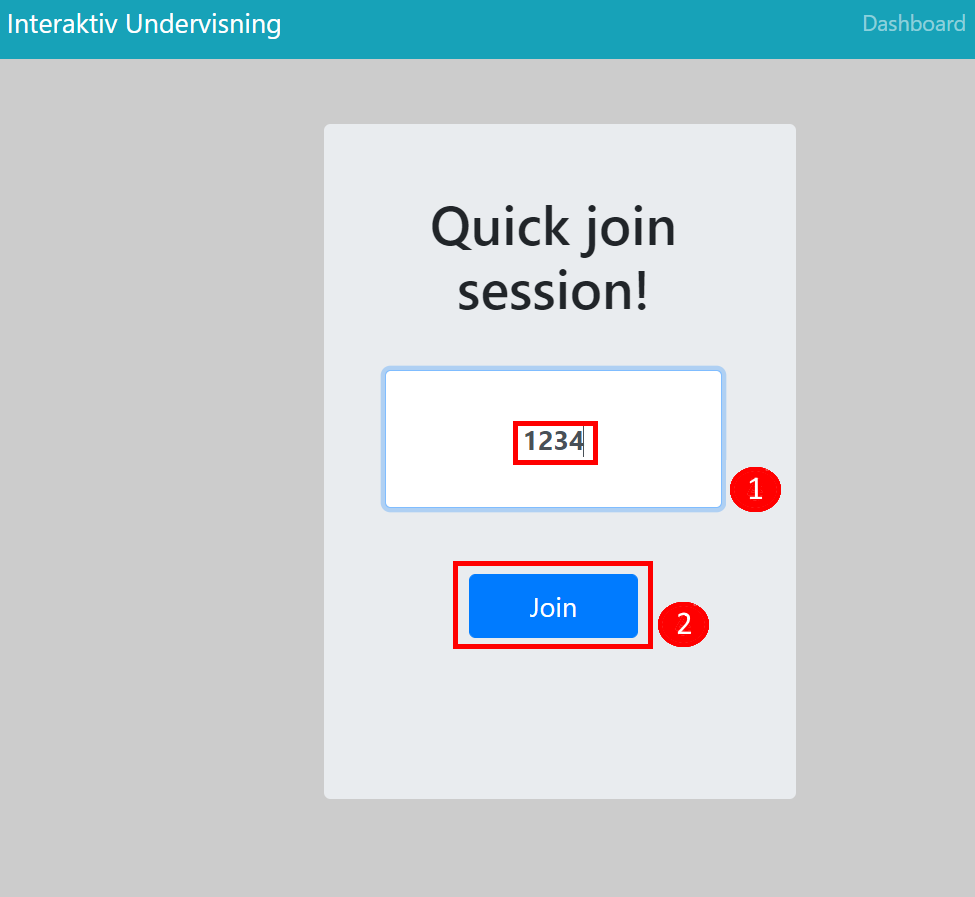
\includegraphics[width=\linewidth]{userManual/joinSession}
		\caption{}
		\label{fig:joinSession}
	\end{subfigure}
	\begin{subfigure}{0.70\linewidth}
		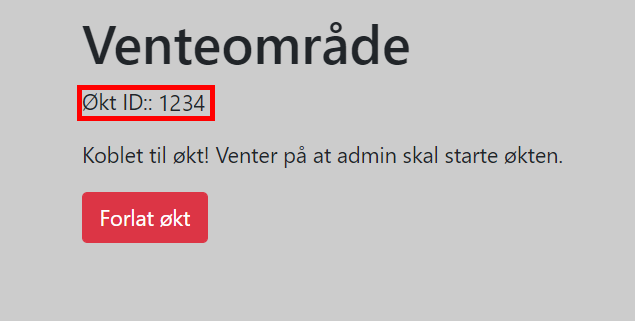
\includegraphics[width=\linewidth]{userManual/waitingRoom}
		\caption{}
		\label{fig:waitingRoom}
	\end{subfigure}
\end{figure}

\begin{userManualItemlist}
	\item[Step I.] Navigate to the dashboard page.
	\item[Step II.] Click the text area within the "Quick join session" area. (1) (Figure: \ref{fig:joinSession})
	\item[Step III.] Write the session code. A session code is 4 characters long. (Figure: \ref{fig:joinSession})
	\item[Step IV.] Click the button (2) labeled "Join" (Figure: \ref{fig:joinSession}) 
	\item[Step V.] If the session exist, you are send to the sessions waiting room. (Figure: \ref{fig:waitingRoom})
\end{userManualItemlist}